% coding:utf-8

%TV-B-Gone
%Copyright (C) 2013, Daniel Winz, Ervin Mazlagic

%This program is free software; you can redistribute it and/or
%modify it under the terms of the GNU General Public License
%as published by the Free Software Foundation; either version 2
%of the License, or (at your option) any later version.

%This program is distributed in the hope that it will be useful,
%but WITHOUT ANY WARRANTY; without even the implied warranty of
%MERCHANTABILITY or FITNESS FOR A PARTICULAR PURPOSE.  See the
%GNU General Public License for more details.
%----------------------------------------

\documentclass[a4paper,
               10pt,
               fleqn]{article}

\author{Ervin Mazlagi\'c, Daniel Winz}
\title{TV-B-Gone}

\usepackage{luxpaper}
\usepackage{luxtitle}
 
\begin{document}
\luxtitle{Papers}
         {TV-B-Gone}
         {Ervin Mazlagi\'c, Daniel Winz}
         {Adligenswil}
         {2012}

\tableofcontents
\newpage

% coding:utf-8

%TV-B-Gone
%Copyright (C) 2013, Daniel Winz, Ervin Mazlagic

%This program is free software; you can redistribute it and/or
%modify it under the terms of the GNU General Public License
%as published by the Free Software Foundation; either version 2
%of the License, or (at your option) any later version.

%This program is distributed in the hope that it will be useful,
%but WITHOUT ANY WARRANTY; without even the implied warranty of
%MERCHANTABILITY or FITNESS FOR A PARTICULAR PURPOSE.  See the
%GNU General Public License for more details.
%----------------------------------------

\section{Einleitung}
Das Ziel dieses Projektes ist es, das ECAD Kicad und die Controllerfamilie 
MSP430 von Texas Instruments kennen zu lernen. 

Dazu wurde ein kleines Projekt gesucht, das sowohl Hardware als auch Firmware 
beinhaltet. Die Entscheidung fiel auf ein TV-B-Gone. Dies ist ein Gerät, das 
in der Lage ist, verschiedene Geräte via Infrarot (z.B. RC-5) auszuschalten. 

Zunächst werden Erfahrungen mit dem MSP430 gesammelt. Als Plattform dazu dient 
das Launchpad von Texas Instruments. 

\part{Allgemeines}
\section{Code Konventionen}
Bei Code-Projekten aller Art ist es wichtig, dass alle Mitglieder gewissen
Style-Konventionen folgen (diese können selbst definiert werden und auch
entgegen allen Empfehlungen sein, jedoch sollten diese einmal aufgesetzt
auch gefolgt werden).

Als Orientierungshilfe kann beispielsweise das Paper von GNU\footnote{
    \emph{GNU coding standards} beschreibt Konventionen im Detail.
    Das Paper ist unter verschiedenen Formaten verfügbar unter 
    \url{http://www.gnu.org/prep/standards/}}
oder das etwas kürzere und überschaubare Paper von Linus Torvalds zur 
Hand genommen werden. Dieses beschreibt die Konventionen zum Kernel-Code
(besonders geeignet da es speziell auf C-Code zugeschnitten ist).

Im folgenden werden die Aussagen aus dem Paper zum Kernel-Style
aufgezeigt.

\subsection{Textbreite}
Der Standard für die Textbreite ist seit jeher 80-Zeichen. Daran sollte
nichts geändert werden. 

\subsection{Encoding}
Aus dem GNU-Paper\footnote{
    GNU coding style, Chapter 5.9 \emph{Character Set}}
geht hervor, dass als erste Wahl das alte 7-Bit ASCII
gilt. Falls man jedoch Zeichen ausserhalb dieses Standards benutzen will
oder muss, ist UTF-8 als erste Wahl zu betrachten.

\subsection{Kommentare}
Kommentare sollten nur mit dem C89-Standard geschrieben werden.

\begin{lstlisting}
/* Das ist eine Main-Funktion */
int main( int argc, char *argv[])
{
    printf("Hallo LuXeria!");
    return 0;
}
\end{lstlisting}

\subsection{Tabs}
Nach (Linus) Kernel-Style sind Tabs 8 Leerzeichen (characters) weit.
Die Überlegung hierzu ist, dass mit grossen Tabs der Code einfacher lesbar
wird und man länger damit arbeiten kann. Kleinere Einzüge erfordern mehr
Konzentration und machen schneller müde bzw. Kopfschmerzen.

Argumente die dagegensprechen sind \emph{``Der Code wird zu Weit auf den
80-Zeichen Terminals und muss gebrochen werden''}. Linus (und andere C 
Coder) meinen, dass C-Code maximal 3 Einzüge haben sollte und entkräften
dieses Argument auf diese Weise\footnote{
    Linux kernel coding style: \emph{``[\dots] if you need more than
    3 levels of indentation, you're screwed anyway, and should fix your 
    program [\dots]''}. Chapter 1}.

\subsection{Klammern}
Als wegweisend gilt der K\&R-Standard, welcher besagt, dass eröffnende
Klammern am Ende der Zeile erfolgen und schliessende zu Beginn und alleine
auf der Zeile stehen. Eine Ausnahme zu dieser Regel gilt bei Funktionen.
Diese sollen ebenfalls eine separate Zeile für die Eröffnende Klammer
haben.

\begin{lstlisting}
if (x != true) {        /* Eröffnende Klammer nach Aufruf */
    y = 0;              
}                       /* Schliessende Klammer alleine */
                        /* aber warum macht man das so?  */
if (x == y) {
    ...
} else if (x > y) {     /* Weil man "Verkettungen" erstellen kann */
    ...                 /* und das ist dann sehr "nice" */
} else {
    ...
}
\end{lstlisting}
\begin{lstlisting}
/* Eine Funktion */
int function(int x)
{
    y = x
    return x;
}
\end{lstlisting}

\subsection{Namensgebung}
\emph{C is a Spartan language} heisst es im Paper von Linus. Was damit
gemeint ist wird im folgenden Beispiel pragmatisch illustriert.

\begin{lstlisting}
/* Naming in languages like Pascal, Java and so on is like */
int ThisVariableIsATemporaryCounter = 0;

/* Where a C Code names like */
int tmp = 0;
\end{lstlisting}

Hier ist allerdings Vorsicht geboten; einfache Namen sollten nur für nicht
globale Variablen genutzt werden. Funktionen und globale Variablen müssen
ersichtlich sein. Schrille Abkürzungen sollten ebenfalls gemieden werden.

\begin{lstlisting}
/* eine Funktion zum Zählen aktiver User sollte z.B. so aussehen */
count_active_user()

/* und nicht etwas so wie */
cntusr()
\end{lstlisting}

Weiter gilt die sogenannte \emph{hungarian notation} als unangebracht.

\subsection{Funktionen}
Als Philosophie zu Funktionen gilt: \emph{``Funktionen sollten kurz und
süss sein, genau eine Sache erledigen und auf ein bis zwei 
Seiten\footnote{
    Eine Seite ist hier nach ISO/ANSI Bildschirmgrösse gemeint, somit 
    80x24 Zeichen gross.} passen. Die Funktion sollte wirklich nur eine 
Sache machen und diese auch gut machen.''}

\subsection{Zusammenfassung}
\begin{itemize}
    \item Textbreite ist 80 Zeichen lang
    \item Encoding ist UTF-8
    \item Kommentare werden in C89-Std. geschrieben 
          d.h. \verb?/* Kommentar */? und nicht \verb?// Kommentar?
    \item Tabs sind 8 Leerzeichen lang
    \item Klammern sind nach K\&R gesetzt (bei Funktionen beide 
          alleinstehend, sonst nur die schliessende alleine)
    \item Globale Namen sind eindeutig, lokale kurz und knapp
    \item Funktionen machen nur eine Sache und machen diese gut
\end{itemize}

% coding:utf-8

%TV-B-Gone
%Copyright (C) 2013, Daniel Winz, Ervin Mazlagic

%This program is free software; you can redistribute it and/or
%modify it under the terms of the GNU General Public License
%as published by the Free Software Foundation; either version 2
%of the License, or (at your option) any later version.

%This program is distributed in the hope that it will be useful,
%but WITHOUT ANY WARRANTY; without even the implied warranty of
%MERCHANTABILITY or FITNESS FOR A PARTICULAR PURPOSE.  See the
%GNU General Public License for more details.
%----------------------------------------

\section{MSP430-Toolchain (unter Linux)}
\subsection{Installation}
Die Installation der MSP-430 Toolchain ist unter Ubuntu bereits in den 
Paketquellen vorhanden (ab Oneric Ocelot aka 11.10)

\begin{itemize}
    \item binutils-msp430 
    \item gcc-msp430 
    \item gdb-msp430 
    \item msp430-libc 
    \item msp430mcu 
    \item mspdebug
\end{itemize}

\noindent
Da hier Pakete verwendet werden, die Manipulationen am GDB vornehmen gilt es
folgende Eingabe zu machen, falls man GDB bereits intalliert hat \\

\verb?apt-get -o Dpkg::Options::="--force-overwrite" install gdb-msp430?

\subsection{Kompilation}
Die Kompilation erfolgt durch \emph{msp430-gcc} und als Option wird der MCU Typ
angegeben (beim MSP430 LaunchPad ist dies \emph{-mmcu=msp430g2553}). Die weiteren
Angaben sind analog zum GCC, d.h. \emph{-o Output-File ./Input-File.c}.
Hier nochmal ein Beispiel \\

\verb?msp430-gcc -mmcu=msp430g2553 -o myprog ./myprog.c?

\subsection{Auf Flash schreiben}
Das Programm wird mittels des MSP-Debugger auf das Flash übertragen. Hierzu
ruft man \emph{mspdebug} und gibt den Treiber an (im Falle des LaunchPad ist
dies der \emph{rf2500}).\\

\verb?mspdebug rf2500?\\

\noindent
Dies eröffnet die Konsole und stellt so viele Kommandos bereit. Um ein 
Übertragen auf das LaunchPad zu ermöglichen, muss der Konsole zuerst das
betreffende Binary angegeben werden.\\

\verb?(mspdebug) prog myprog?\\

\noindent
Nachdem der Debugger das Binary kennt, schreibt er es sofort auf den Flash.
Damit das Programm ausgeführt wird, muss dem Debugger noch das Kommando 
\emph{run} übergeben werden.\\

\verb?(mspdebug) run?

\subsection{Debug \& Simulation}
\emph{mspdebug} bietet wie es der Name schon verrät Debug-Möglichkeiten.
Hierzu wird \emph{mspdebug} mit der Option \emph{sim} ausgeführt und
dann in dessen Konsole \emph{gdb} eingegeben.

\subsection{Quellen \& Testing}
Die hier angegebenen Informationen sind ein Auszug aus dem Artikel
\href{http://wiki.ubuntuusers.de/MSP430-Toolchain}{MSP-430 Toolchain} von 
Ubuntuusers. 

Die hier oben genannten Anleitungen sind mit folgender Konfiguration
erfolgreich gestestet worden an einem MSP-EXP430G2 LaunchPad Rev 1.5\footnote{
    Für Luxeria LuXeria-Member stehen mehrere MSP430-LaunchPads und eine
    EZ430-Chronos frei zur Verfügung im LuXlab.}:

\begin{table}[h!]
\centering
\begin{tabular}{ l l }
Hardware        & Lenovo ThinkPad 430 \\
Kernel-Name     & Linux \\
Kernel-Release  & 3.5.0-17-generic \\
Kernel-Version  & \#28-Ubuntu SMP Tue Oct 9 19:32:08 UTC 2012 \\
Machine         & i686 \\
Operatin System & GNU/Linux\\
\end{tabular}
\end{table}

\section{MSP430-Toolchain (unter Windows)}
\subsection{Installation}
Diese Anleitung befasst sich nur mit mspgcc. Entwicklungsumgebungen wie Eclipse 
werden nicht behandelt. 
\subsubsection{Download}
Die Installation ist unter Windows etwas umständlicher als unter Linux. 
Zunächst muss der mspgcc \footnote{\url{http://sourceforge.net/projects/mspgcc/
files/Windows/mingw32/}} und der msp430-gdbproxy \footnote{\url{http://
sourceforge.net/projects/mspgcc/files/Outdated/msp430-gdbproxy/2006-11-14/}} 
heruntergeladen werden. 

Aktueller als msp430-gdbproxy ist die Installation von MSPdebug. Dies wird an 
dieser Stelle zu einem späteren Zeitpunkt erläutert. 

Ausserdem müssen noch die beiden DLLs MSP430.dll und HIL.dll heruntergeladen 
werden. Diese findet man unter \footnote{\url{http://software-dl.ti.com/msp430/
msp430_public_sw/mcu/msp430/DLLv2/latest/index_FDS.html}}. Um diese jedoch 
herunterladen zu können muss man bei Texas Instruments registriert sein. Eine 
andere Möglichkeit um an die fehlenden DLLs zu gelangen ist die Installation 
der Kickstartversion von IAR Embedded Workbench von \footnote{\url{http://
processors.wiki.ti.com/index.php/IAR_Embedded_Workbench_for_TI_MSP430}}. Dazu 
ist keine Anmeldung erforderlich. 

Zudem wird der Treiber aus slac254 von \footnote{\url{?}} benötigt. 

\subsubsection{Installation Treiber}
Als Erstes muss der Treiber für das Launchpad installiert werden. Dazu muss 
slac524 entpackt werden. Anschliessend muss LaunchPad\_Driver.exe ausgeführt 
werden. Unter Windows 7 muss LaunchPad\_Driver.exe als Administrator ausgeführt 
werden. 

Wenn nun das Launchpad angeschlossen wird, muss es im Gerätemanager als 
serielle Schnittstelle angezeigt werden. 


% Die Installation der MSP-430 Toolchain ist unter Ubuntu bereits in den 
% Paketquellen vorhanden (ab Oneric Ocelot aka 11.10)

% \begin{itemize}
%     \item binutils-msp430 
%     \item gcc-msp430 
%     \item gdb-msp430 
%     \item msp430-libc 
%     \item msp430mcu 
%     \item mspdebug
% \end{itemize}

% \noindent
% Da hier Pakete verwendet werden, die Manipulationen am GDB vornehmen gilt es
% folgende Eingabe zu machen, falls man GDB bereits intalliert hat \\

% \verb?apt-get -o Dpkg::Options::="--force-overwrite" install gdb-msp430?

% \subsection{Kompilation}
% Die Kompilation erfolgt durch \emph{msp430-gcc} und als Option wird der MCU Typ
% angegeben (beim MSP430 LaunchPad ist dies \emph{-mmcu=msp430g2553}). Die weiteren
% Angaben sind analog zum GCC, d.h. \emph{-o Output-File ./Input-File.c}.
% Hier nochmal ein Beispiel \\

% \verb?msp430-gcc -mmcu=msp430g2553 -o myprog ./myprog.c?

% \subsection{Auf Flash schreiben}
% Das Programm wird mittels des MSP-Debugger auf das Flash übertragen. Hierzu
% ruft man \emph{mspdebug} und gibt den Treiber an (im Falle des LaunchPad ist
% dies der \emph{rf2500}).\\

% \verb?mspdebug rf2500?\\

% \noindent
% Dies eröffnet die Konsole und stellt so viele Kommandos bereit. Um ein 
% Übertragen auf das LaunchPad zu ermöglichen, muss der Konsole zuerst das
% betreffende Binary angegeben werden.\\

% \verb?(mspdebug) prog myprog?\\

% \noindent
% Nachdem der Debugger das Binary kennt, schreibt er es sofort auf den Flash.
% Damit das Programm ausgeführt wird, muss dem Debugger noch das Kommando 
% \emph{run} übergeben werden.\\

% \verb?(mspdebug) run?

% \subsection{Debug \& Simulation}
% \emph{mspdebug} bietet wie es der Name schon verrät Debug-Möglichkeiten.
% Hierzu wird \emph{mspdebug} mit der Option \emph{sim} ausgeführt und
% dann in dessen Konsole \emph{gdb} eingegeben.

\subsection{Quellen \& Testing}
Die hier angegebenen Informationen sind ein Auszug aus dem Artikel
\href{http://springuin.nl/articles/launchpadwindows}{TI LaunchPad on Windows} von 
Springuin. 

% Die hier oben genannten Anleitungen sind mit folgender Konfiguration
% erfolgreich gestestet worden an einem MSP-EXP430G2 LaunchPad Rev 1.5\footnote{
%     Für Luxeria LuXeria-Member stehen mehrere MSP430-LaunchPads und eine
%     EZ430-Chronos frei zur Verfügung im LuXlab.}:

\begin{table}[h!]
\centering
\begin{tabular}{ l l }
Hardware        & HP ProBook 4740s \\
Betriebssystem  & Windows 7 Professional 64 Bit \\
                & Service Pack 1 \\
% Kernel-Release  & 3.5.0-17-generic \\
% Kernel-Version  & \#28-Ubuntu SMP Tue Oct 9 19:32:08 UTC 2012 \\
% Machine         & i686 \\
% Operatin System & GNU/Linux\\
\end{tabular}
\end{table}


% coding:utf-8

%TV-B-Gone
%Copyright (C) 2013, Daniel Winz, Ervin Mazlagic

%This program is free software; you can redistribute it and/or
%modify it under the terms of the GNU General Public License
%as published by the Free Software Foundation; either version 2
%of the License, or (at your option) any later version.

%This program is distributed in the hope that it will be useful,
%but WITHOUT ANY WARRANTY; without even the implied warranty of
%MERCHANTABILITY or FITNESS FOR A PARTICULAR PURPOSE.  See the
%GNU General Public License for more details.
%----------------------------------------

\section{Einfaches Hello World}
Nachfolgend wird ein einfaches Hello World Schritt für Schritt erläutert. 
\begin{lstlisting}
/* Example-Code from http://wiki.ubuntuusers.de/MSP430-Toolchain */

#include  <msp430.h>                      /*  */  

int main(void)
{
        WDTCTL = WDTPW + WDTHOLD;         /* Stop watchdog timer */
        DCOCTL    = CALDCO_16MHZ;         /* Initializes clock */
        BCSCTL1   = XT2OFF|CALBC1_16MHZ;    /* module for 16 MHz*/
        BCSCTL2   = 0;           
        BCSCTL3   = 0;           
        P1DIR = BIT0 | BIT6;              /* P1.0 and P1.6 output */
                                            /* red and green LED */
        P1OUT = BIT0;                     /* red LED on */

        for (;;)                          /* Loop forever */
        {
                volatile unsigned long i;
                P1OUT ^= BIT0 | BIT6;     /* Toggle LEDs with XOR */
                i = 99999;                /* Delay */

                do (i--);                 /* busy waiting (bad) */
                while (i != 0);
        }
}

\end{lstlisting}

\part{Dokumentation}
% coding:utf-8

%TV-B-Gone
%Copyright (C) 2013, Daniel Winz, Ervin Mazlagic

%This program is free software; you can redistribute it and/or
%modify it under the terms of the GNU General Public License
%as published by the Free Software Foundation; either version 2
%of the License, or (at your option) any later version.

%This program is distributed in the hope that it will be useful,
%but WITHOUT ANY WARRANTY; without even the implied warranty of
%MERCHANTABILITY or FITNESS FOR A PARTICULAR PURPOSE.  See the
%GNU General Public License for more details.
%----------------------------------------

\section{Anforderungen}
Es soll ein Gerät entwickelt werden, mit welchem Geräte verschiedener 
Hersteller , die über eine Infrarotschnittstelle verfügen ausgeschaltet 
werden können. Dabei sollen folgende Anforderungen erfüllt werden: 

\begin{table}[h!]
  \begin{tabular}{@{}p{0.3\textwidth}p{0.2\textwidth}p{0.2\textwidth}}
    \rowcolor{white} \textbf{Anforderung}     & \textbf{Pflicht} & \textbf{Wunsch}\\
                                              &                  &                \\
    \rowcolor{white} Speisung                 & 3V Lithium Zelle &                \\
    \rowcolor{white}                          &                  & Externe Spannung\\
    \rowcolor{lgray} Protokolle               & RC-5             &                \\
    \rowcolor{lgray}                          &                  & Revox          \\
    \rowcolor{white} Stromverbrauch Stand-by  & $\leq$100$\mu$A  & $\leq$10$\mu$A \\
    \rowcolor{lgray} Stromverbrauch Betrieb   & $\leq$50mA       & $\leq$20mA     \\
  \end{tabular}
%   \caption{Anforderungen}
  \label{tab:anforderungen}
\end{table}

\section{RC5}
Im Folgenden sollen alle wichtigen Facts zu und über RC5 gegeben werden.

\subsection{Protokoll}
Hier die wichtigsten Facts 
\begin{itemize}
    \item Codelänge beträgt 24.889ms
    \item Pause zwischen Wiederholungen beträgt 88.889ms
    \item Code ist \emph{biphase}-coded\footnote{
        \emph{biphase-coded} kann frei als Flankengetriggert übersetzt
        werden. Siehe Codebeispiel im Bild \ref{pic:rc5_simple} }
    \item Code besteht aus 14-Bit Word
    \begin{itemize}
        \item 2 Start Bits
        \item 1 Toggle Bit
        \item 5 Systemadress-Bits
        \item 6 Kommando-Bits
    \end{itemize}
\end{itemize}

\begin{figure}[h!]
    \centering
    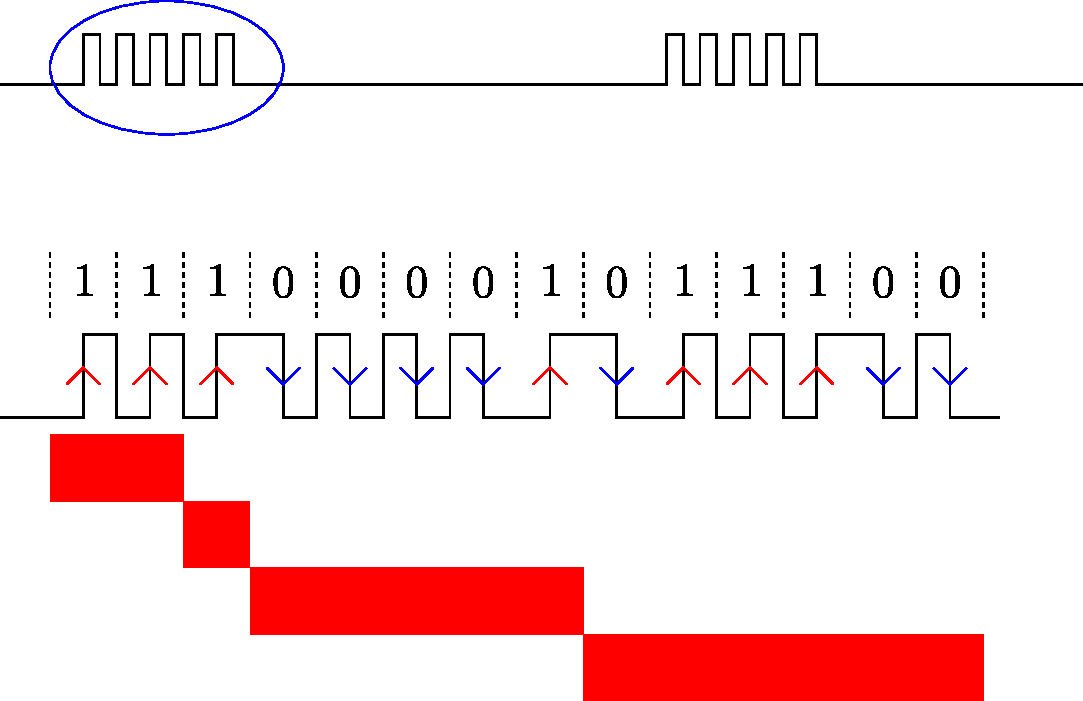
\includegraphics[width=0.8\textwidth]{rc5_simple.pdf}
    \label{pic:rc5_simple}
    \caption{RC5 Protokoll}
\end{figure}

\subsubsection{Start-Bits}
Das Startsignal besteht aus zwei Bits. Zuerst das eigentliche Start-Bit
und dann das sogenannte Field-Bit. Das Startbit ist immer logisch 1 und
stellt beim Empfänger die Verstärkung ein zum einlesen der Daten.
Das Field-Bit wird verwendet um dem Empfänger mitzuteilen, ob man den
unteren (0-63) oder oberen (64-127) Kommandobereich verwendet.
\subsubsection{Toggle-Bit}
Das Toggle- oder auch Steuer-Bit wird dazu verwendet permanentes (bzw. 
wiederholendes) senden von neuem Senden zu unterscheiden.
Dies ist nützlich um z.b. zu erkennen ob eine Taste dauerhaft gedrückt ist
bei der Fernbedienung etc.
\subsubsection{Systemadress-Bits}
Die 5 Systemadress-Bits erlauben es zwischen 32 verschiedenen Geräten
zu operieren.
\subsubsection{Kommando-Bits}
Die 6 Kommando-Bits bieten ein Set von 64 Befehlen an, mit welchem ein
Gerät (welches mit den 5 Systemadress-Bits spezifiziert wurde) angesteuert
werden kann.

\subsection{System-Adressen}

\begin{table}[h!]
    \footnotesize
    \centering
    \begin{tabular}{c l c l c l c l}
    Adresse & Gerät & Adresse & Gerät & Adresse & Gerät & Adresse & Gerät 
    \\
    \hline &&&&&&& \\
    00      & TV1       & 08 & Sat.-Rec 1   & 16 & Audio-PreAmp 1       & 24 & -                \\
    01      & TV2       & 09 & Camera       & 17 & Reciever/Tuner       & 25 & -                \\
    02      & Teletext  & 10 & Sat.-Rec 2   & 18 & Audio Tape Rec.      & 26 & CDR              \\
    03      & Video VD  & 11 & -            & 19 & Audio PreAmp 2$^*$   & 27 & -                \\
    04      & Video LV1 & 12 & Video-CD     & 20 & CD-Player            & 28 & -                \\
    05      & VCR1      & 13 & Camcorder    & 21 & Plattenspieler       & 29 & Beleuchtung 1    \\
    06      & VCR2      & 14 & -            & 22 & -                    & 30 & Beleuchtung 2    \\
    07      & exp.      & 15 & -            & 23 & DAT-T./MD-Rec.       & 31 & Telefon          \\
    \end{tabular}
    \caption{RC5 Systemadressen}
    \label{tab:rc5_systemadressen}
\end{table}


\begin{appendix}
    \clearpage
    \pagenumbering{roman}
    \newpage

    \section{Linux Kernel Coding Style}
    Link zum ganzen Dokument 

    \href{https://computing.llnl.gov/linux/slurm/coding_style.pdf}{
        Linux Kernel Coding Style}
    \begin{figure}[h!]
    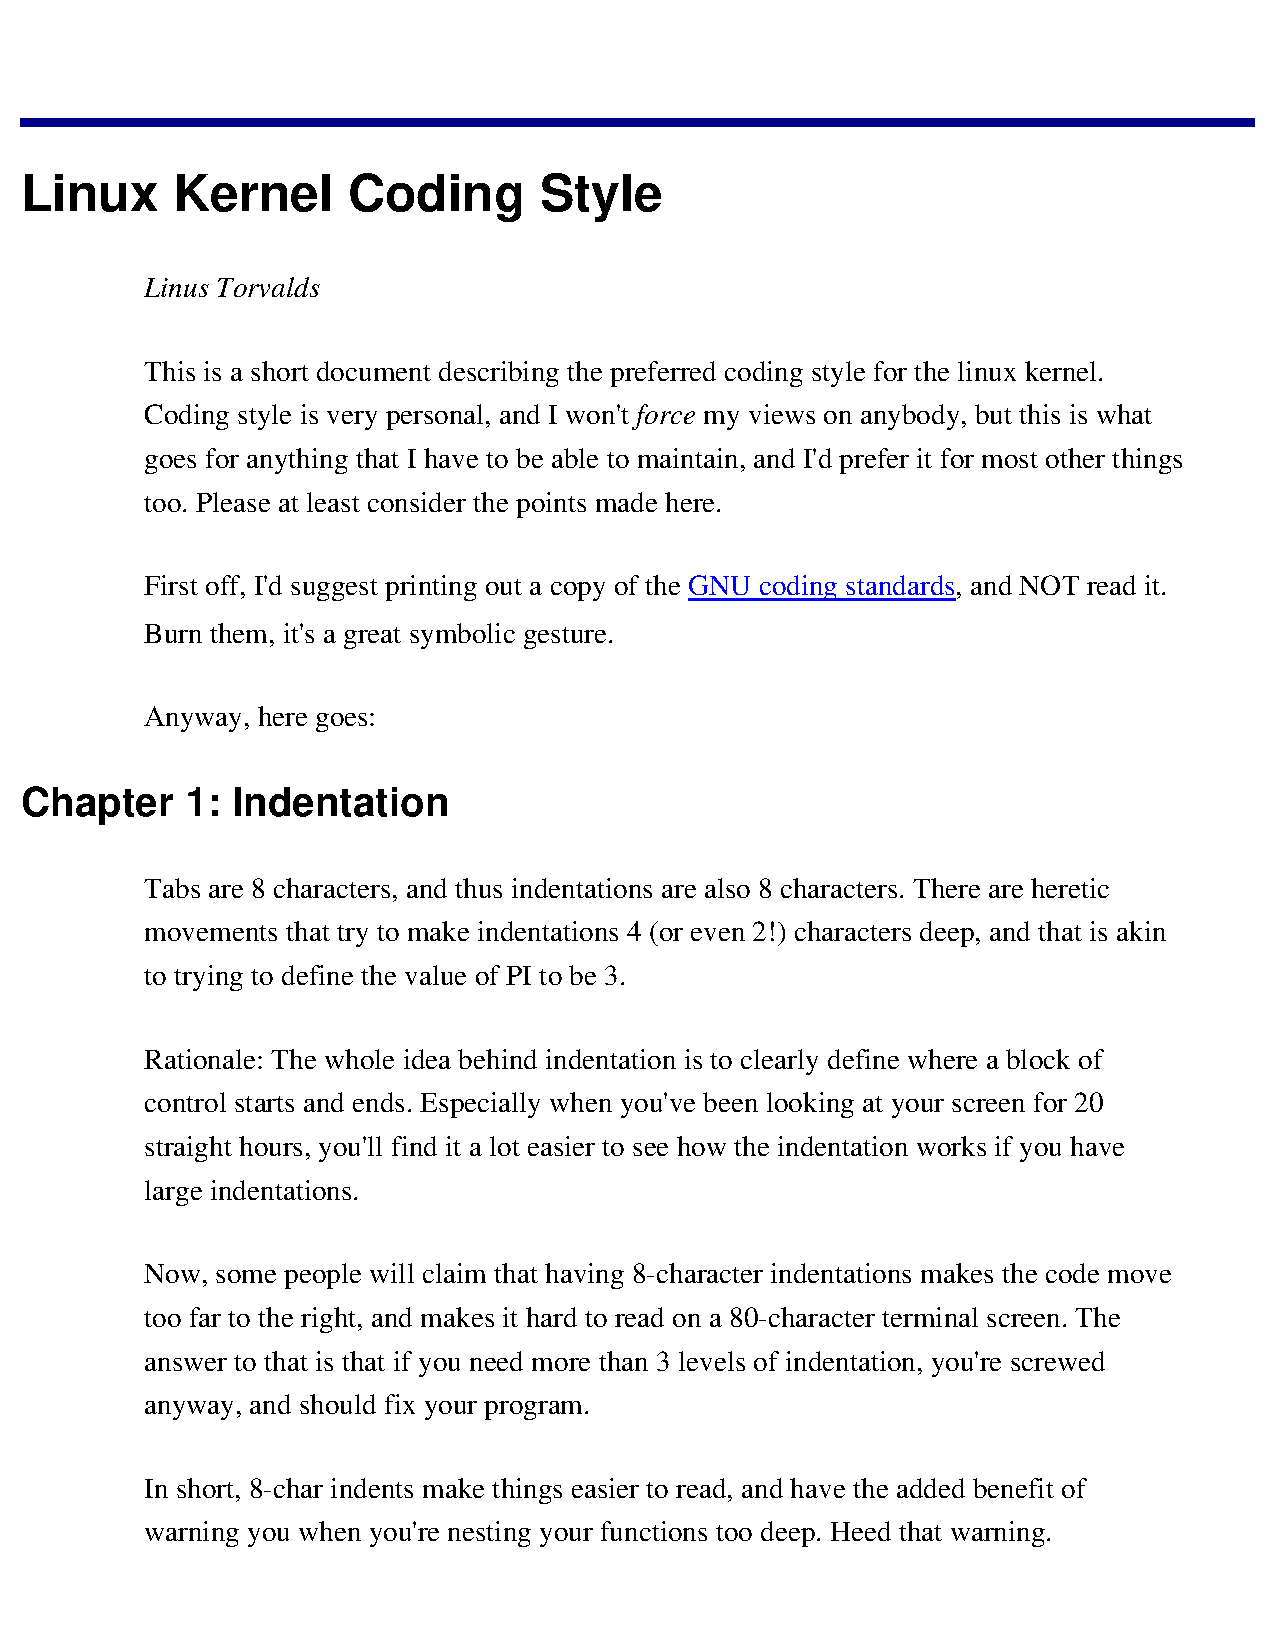
\includegraphics[page=1, width=1\textwidth]{kernelstyle.pdf}
    \end{figure}
    \newpage

    \section{GNU Coding Standards}
    Link zum ganzen Dokument
    \href{http://www.gnu.org/prep/standards/}{GNU Coding Standards}
    \begin{figure}[h!]
    \includegraphics[page=5, width=1\textwidth]{gnustandard.pdf}
    \end{figure}
\end{appendix}

\end{document}

